\chapter{Docker-Anwendungsszenarien für den Softwareentwickler}
\label{cha:szenarien}
Dieses Kapitel zeigt exemplarisch mögliche Anwendungsfälle für die Verwendung von Docker als Werkzeug für Softwareentwickler und wie diese bei ihren alltäglichen Tätigkeiten unterstützen werden können.

Das Entwickeln von Software erfordert die Installation zahlreicher Werkzeuge.
Wenn sich diese auf lediglich ein Projekt beschränkt, stellt dies kein Problem dar, da es zu keinen Versionsinkompatibilitäten kommt und die Werkzeuge nicht laufend gewechselt werden müssen.
Werden allerdings mehrere Projekte parallel entwickelt und zusätzlich noch Beiträge zu Open-Source-Projekten geleistet, wird dieses Unterfangen erheblich komplizierter.
Unterschiedliche Laufzeitumgebungen, Compiler-Versionen, Build-Werkzeuge und Frameworks führen sehr schnell zu einem unüberschaubaren und instabilen System \autocite{smashing-local-devenv-docker:online}.

In \autocite{smashing-local-devenv-docker:online} werden die bestehenden Lösungen für die auftretenden Probleme aufgelistet:
\begin{itemize}
    \item Anstatt Abhängigkeiten auf Systemebene zu installieren werden diese von \emph{Paketmanagern} auf Projektebene verwaltet.
    Vertreter davon sind zum Beispiel npm\footnote{\url{https://www.npmjs.com/}} für JavaScript, Maven\footnote{url{https://maven.apache.org/}} für Java oder NuGet\footnote{\url{https://www.nuget.org/}} für .NET.
    \item Zusätzlich zu Paketen müssen allerdings auch die Laufzeitumgebungen verwaltet werden.
    Bei unterschiedlichen Projekten können unterschiedliche Versionen dieser benötigt werden, wodurch Werkzeuge wie der Node Version Manager (nvm\footnote{\url{https://github.com/creationix/nvm}}) oder der Ruby Version Manager (RVM\footnote{\url{https://rvm.io/}}) entstanden sind.
    Diese müssen allerdings auf dem Entwicklerrechner verwaltet werden und erschweren den schnellen Wechsel zwischen unterschiedlichen Projekten.
    Bei alten Legacy-Systeme ist eine Unterstützung durch diese Werkzeuge außerdem nicht garantiert.
    \item Mit dem Aufschwung der Virtualisierung und Werkzeugen wie Vagrant wurden viele dieser Probleme gelöst.
    Allerdings ist die Notwendigkeit einer virtuellen Maschine pro Projekt sehr ressourcen- und wartungsintensiv.
    Ein weiterer Nachteil ist, dass Vagrant auf Entwicklerrechner ausgelegt ist und dadurch nicht garantiert werden kann, dass die entwickelte Software auch auf dem Produktionssystem läuft \autocite{laradock-docs:online}.
\end{itemize}
Docker bietet eine Abstraktion des Betriebssystems und die Möglichkeit, die benötigten Komponenten einer Anwendung deklarativ zu beschreiben.
Dadurch ist es möglich, die Laufzeitumgebung und die benötigten Komponenten der Anwendung gemeinsam mit dieser im Versionsverwaltungssystem aufzubewahren.
Danach ist lediglich Docker die Voraussetzung dafür, dass mit einem plattformübergreifenden Kommando mit der Entwicklung von Software begonnen werden kann.

Travis Reeder liefert in seinem Blogeintrag über die Entwicklung mit Docker (\autocite{why-docker-for-development:online}) folgende Gründe für die Verwendung von Docker für Softwareentwickler:
\begin{itemize}
    \item Die Entwicklungsumgebung ist nicht vom Betriebssystem oder dessen Version abhängig. Unterschiedliche Personen im Team können problemlos auf Windows, macOS und Linux gemeinsam an einem Produkt arbeiten. Dieser Aspekt ist besonders bei der Entwicklung von Open-Source-Projekten wichtig, da dort unzählige Entwickler ohne zentrale Verwaltung zu einem Produkt beitragen.
    \item Die Entwicklungs- und Produktionsumgebung werden vereinheitlicht. Quelltext, der in der Entwicklungsumgebung getestet ist, funktioniert automatisch auch auf dem Produktivsystem.
    \item Komplizierte Build-Prozesse können abstrahiert werden, sodass die Entwickler diesen nicht verstehen müssen. Außerdem kann dieser Prozess separat entwickelt und getestet oder sogar wiederverwendet werden.
    \item Unterschiedliche Laufzeitumgebungen haben keinen Einfluss auf das Hostsystem des Entwicklers. Besonders die Entwicklung von Java, Ruby, Python und Node wird dadurch stark vereinfacht. Zusätzlich ist es beispielsweise einfach möglich, die Software mit einer anderen Compiler-Version zu übersetzen, um zu überprüfen, ob diese kompatibel ist.
    \item Das Veröffentlichen der Software wird einfacher. Es muss lediglich ein Container der Anwendung erstellt werden, der nun auf jedem Docker-Host lauffähig ist.
    \item Es müssen keine besondere IDE verwendet oder Kommandos über SSH auf einer virtuellen Maschine ausgeführt werden. Der Container wird in das Host-System integriert und ist beinahe nicht sichtbar.
    \item Entwicklern wird ein schnellerer und einfacher Einstieg in ein Projekt ermöglicht, da große Teile des Entwicklungsprozesses abstrahiert werden. Diese muss der Entwickler anfangs nicht verstehen, wodurch die Lernkurve und dadurch auch die Einarbeitungszeit sinken.
\end{itemize}


\section{Softwareevaluierung}
\label{sec:softwareevaluierung}
Die Evaluierung und Auswahl von Werkzeugen, Frameworks und Komponenten eines Softwaresystems ist eine wichtige Aufgabe des Softwareentwicklers.
Ein sehr mühsamer Aspekt dieser Tätigkeit ist das Einarbeiten und Verstehen der Installation und Konfiguration der zu evaluierenden Werkzeuge.
Außerdem werden oftmals unnatürliche Standardpfade (beispielsweise \verb$C:\xampp$ bei der Installation der PHP-Umgebung xampp\footnote{\url{https://www.apachefriends.org/}}) gewählt, oder die Deinstallation von getesteten Werkzeugen hinterlässt Spuren am Host-System des Softwareentwicklers.
Ein weiteres Problem können fehlende Benutzerrechte darstellen, wodurch die Evaluierung bestimmter Werkzeuge gar nicht möglich ist.

\subsubsection{Beispiel: ArangoDB}
Docker ermöglich ein sehr schnelles Testen von Datenbanken, Anwendungsservern und anderen Werkzeugen.
Außerdem wird beim Löschen eines Containers das System automatisch wieder auf einen "`sauberen"' Ausgangszustand zurückgesetzt.
Diese Möglichkeit kann sogar zu Marketingzwecken verwendet werden, wie auf der Homepage von ArangoDB\footnote{\url{https://www.arangodb.com/}} in \cref{fig:arangodb-docker-marketing} dargestellt ist.

Das dort verwendete Kommando ist aus Marketinggründen allerdings etwas zu einfach gehalten.
Würde der Container auf diese Weise gestartet werden, wäre der Netzwerk-Port auf dem Host-System nicht sichtbar und es kann kein Zugriff auf die Datenbank stattfinden.
In \cref{lst:docker-run-arangodb} ist das komplette Startkommando dargestellt.
\cref{fig:arangodb-demo} zeigt die Administrationsoberfläche der gestarteten Datenbank.

Sobald der Container gestoppt wird, wird er durch \texttt{--rm} wieder gelöscht und es verbleiben keine Reste aus der Evaluierungsphase auf dem Host-System.
Ein zusätzlicher Vorteil der Verwendung von Docker ist, dass genau derselbe Container auch im Produktivsystem verwendet werden kann.
Dies ermöglicht beispielsweise die rasche Weiterentwicklung von Prototypen.

\begin{figure}[htbp]
    \centering
    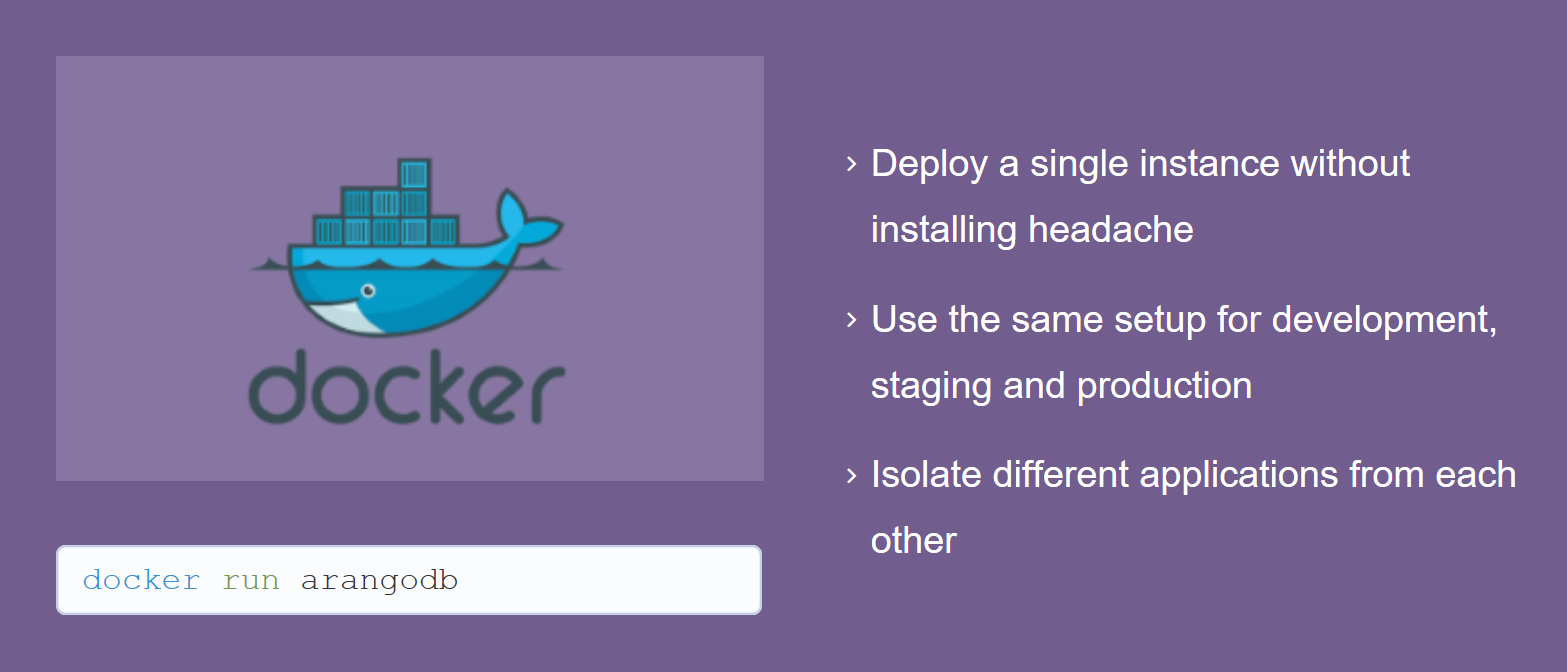
\includegraphics[width=0.7\linewidth,clip]{images/arangodb-docker-marketing}
    \caption{Docker als Marketinginstrument bei ArangoDB}
\label{fig:arangodb-docker-marketing}
\end{figure}

\begin{lstlisting}[caption=Docker-Kommando zum Starten von ArangoDB, language=bash, label=lst:docker-run-arangodb]
docker run --rm -d -e ARANGO_NO_AUTH=1 -p 8529:8529 arangodb
\end{lstlisting}

\begin{figure}[htbp]
    \centering
    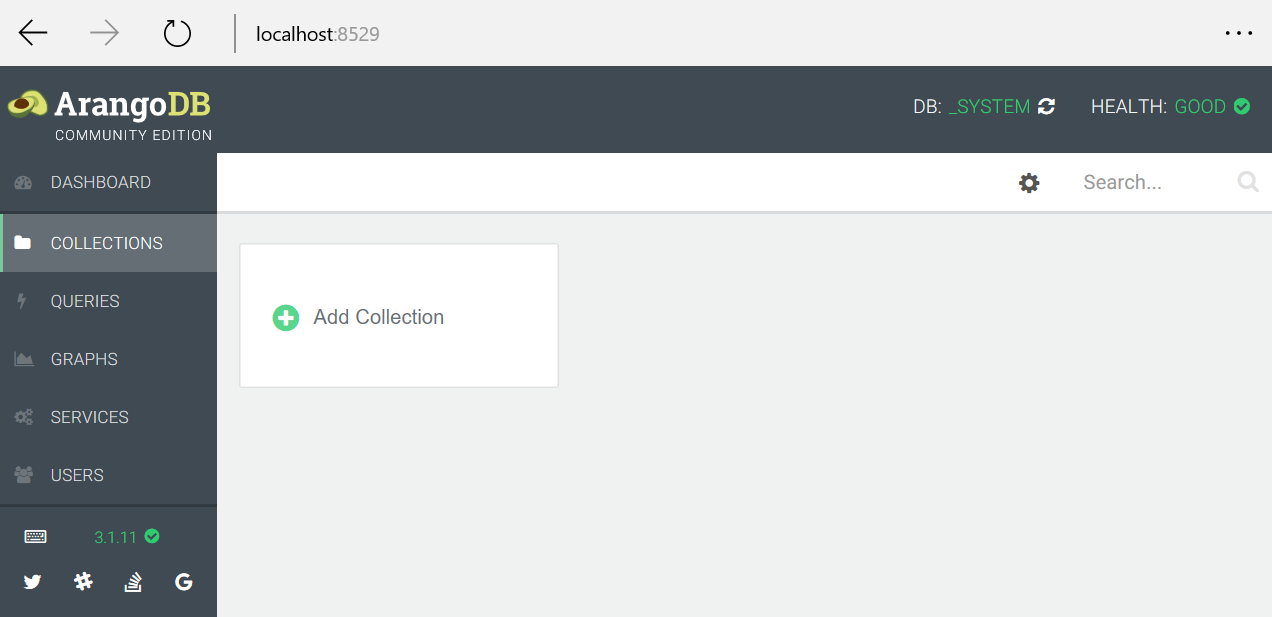
\includegraphics[width=0.8\linewidth,clip]{images/arangodb-demo}
    \caption{ArangoDB als Docker-Container}
\label{fig:arangodb-demo}
\end{figure}

\section{Plattformunabhängige CLI-Anwendungen}
\label{sec:cross-platform-applications}
In \autocite{docker-cli-tools:online} beschreibt Mike English die Möglichkeit Docker als Laufzeitumgebung für Kommandozeilenwerkzeuge zu verwenden.
Durch die Bündelung der Abhängigkeiten und des Werkzeugs werden bei der Verwendung von Docker keine Laufzeitsysteme auf dem Host benötigt.
Dies führt besonders bei Python und Ruby zur Vermeidung von Versionsproblemen und der einfacheren Verwendung auf Windows.
Außerdem bietet der Docker Hub eine sehr angenehme Möglichkeit für die Veröffentlichung des Werkzeuges.
Dem gegenüber stehen die Systemvoraussetzung Docker und die damit verbundene Imagegröße aufgrund der Docker-Basisimages.

\subsubsection{Beispiel: Jekyll}
Jekyll\footnote{\url{https://jekyllrb.com/}} ist ein in Ruby geschriebener Generator für statische Webseiten.
In der offiziellen Dokumentation ist beschrieben, dass Windows keine offiziell unterstützte Plattform sei, es aber trotzdem folgende Möglichkeit zur Installation gibt \autocite{jekyll-windows:online}:
\begin{enumerate}
    \item Installieren eines Paketmanagers wie beispielsweise Chocolatey\footnote{\url{https://chocolatey.org/}}.
    \item Installieren von Ruby mit Chocolatey: \texttt{choco install ruby -y}.
    \item Installieren von Jekyll: \texttt{gem install jekyll}.
\end{enumerate}
Für die Installation eines Werkzeuges werden also zwei weitere Abhängigkeiten benötigt, wobei die Plattform weiterhin als "`nicht offiziell unterstützt"' wird.

Allerdings bietet Jekyll auch ein vorgefertigtes offizielles Docker-Image\footnote{\url{https://hub.docker.com/r/jekyll/jekyll/}} an, welches mit dem in \cref{lst:docker-run-jekyll} beschriebenen Kommando Jekyll im aktuellen Ordner startet.
Danach ist die Webseite unter \url{http://localhost:4000} erreichbar.

Die Verwendung von Jekyll konnte auf diese Weise anstatt der dreistufigen Installation auf das Starten eines Containers reduziert werden.

\begin{lstlisting}[caption=Docker-Kommando zum Starten von Jekyll, language=bash, label=lst:docker-run-jekyll]
docker run -it --rm -v ${pwd}:/srv/jekyll -p 4000:4000 jekyll/jekyll /usr/local/bin/jekyll serve
\end{lstlisting}

\subsubsection{Beispiel: mdp}
Im vorigen Beispiel wurde ein bereits verwendetes Docker-Image als plattformunabhängiges Werkzeug verwendet.
Da allerdings nicht für jedes Werkzeug ein Docker-Image besteht, ist in \cref{lst:dockerfile-mdp} ein Dockerfile abgebildet, das die Portierung eines existierenden Werkzeuges für Docker zeigt.
In diesem Fall handelt es sich dabei um mdp\footnote{\url{https://github.com/visit1985/mdp}}, dieses Verfahren kann aber auf jedes Linux-Kommandozeilenwerkzeug angewendet werden.

mdp ist ein C Programm, das aus Markdown-Dateien Folien für die Kommandozeile erstellt.
Im Dockerfile werden wie in der offiziellen Dokumentation die Übersetzung und Installation make durchgeführt.
Das Startkommando ist für eine möglichst intuitive Verwendung wie in \cref{sec:container-startup-command} beschrieben definiert.
Wird keine Präsentation übergeben, startet der Container mit einer Demo-Präsentation, die die Verwendung von mdp erklärt.

\lstinputlisting[caption=Docker-Image für mdp,label={lst:dockerfile-mdp}]{listings/Dockerfile.mdp}

\subsubsection{Aufruf aus der Powershell}
Die Abstraktion von Kommandozeilenanwendungen mit Docker bietet, wie in den beiden Beispielen gesehen, zahlreiche Vorteile.
Doch ein komplettes Docker-Run-Kommando zum Starten einer Anwendung ist nicht nur sehr umständlich und fehleranfällig, sondern verlangt auch bei jedem Start die Konfiguration zahlreicher Parameter.

Mithilfe von Shell-Aliasen oder Powershell-Funktionen lässt sich dieses Problem allerdings sehr einfach lösen.
In \cref{lst:powershell-functions} sind die zwei Funktionen zum vereinfachten Starten von Jekyll und mdp aufgelistet.
\texttt{-v \$\{pwd\}:...} ermöglicht dem Container das Arbeiten mit dem aktuellen Ordner, indem es diesen an den Container bindet.
Mithilfe von \texttt{\$\{args\}} werden die Parameter des Funktionsaufrufes an den Docker-Container weitergeleitet.

Der Aufruf der Werkzeuge erfolgt nun wie gewohnt, wobei die Ausführung in einem Docker-Container für den Anwender unsichtbar wird.

\begin{lstlisting}[caption=Powershell-Funktionen für Docker-Kommandos, language=bash, label=lst:powershell-functions]
$ jekyll
function jekyll { docker run -it --rm -v ${pwd}:/srv/jekyll -p 4000:4000 jekyll/jekyll /usr/local/bin/jekyll ${args} }
function mdp { docker run -it --rm -v ${pwd}:/data bemayr/mdp mdp ${args} }
\end{lstlisting}

\begin{lstlisting}[caption=Automatische Installation der Docker-basierten CLI-Anwendungen, language=bash, label=lst:docker-auto-install-cli]
$ jekyll
Unable to find image 'jekyll/jekyll:latest' locally
latest: Pulling from jekyll/jekyll
baf40e071063: Pull complete
70acac711d95: Downloading [======>       ] 11.33 MB/91.37 MB
...
\end{lstlisting}


\section{Containerbasierte Integrationstests}
\label{sec:containerbasiertes-integrationstests}
% - https://hharnisc.github.io/2016/06/19/integration-testing-with-docker-compose.html
% - https://engineering.gosquared.com/testing-with-docker

\section{Plattformübergreifende Übersetzung}
\label{sec:plattformuebergreifende-uebersetzung}
\subsubsection{Beispiel: gcc}
\begin{lstlisting}[caption=Docker-Kommando zum Übersetzen eines C-Programmes mit gcc, language=bash, label=lst:docker-run-gcc]
docker run --rm -v ${pwd}:/usr/src -w /usr/src frolvlad/alpine-gcc gcc -o greet greet.c
\end{lstlisting}

\begin{figure}[htbp]
    \centering
    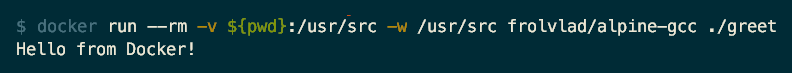
\includegraphics[width=0.8\linewidth,clip]{images/greet-output}
    \caption{Hello-World-Ausgabe unter Linux}
\label{fig:greet-output}
\end{figure}

https://github.com/dockcross/dockcross

\begin{lstlisting}[caption=Kommandos zum Kompilieren mit dockcross, language=bash, label=lst:dockercross-arm-greet]
cd ~/src/dockcross
docker run --rm dockcross/linux-armv7 > ./dockcross-linux-armv7
chmod +x ./dockcross-linux-armv7
./dockcross-linux-armv7 bash -c '$CC test/C/greet.c -o greet_arm'
\end{lstlisting}

\section{IDE as a Container}
\label{sec:ideasacontainer}
https://github.com/JAremko

\subsubsection{Beispiel: vim (jare/vim-bundle)}
\begin{lstlisting}[caption=Docker-Kommando zum Starten von vim, language=bash, label=lst:docker-run-vim]
$ docker run -it --rm -v ${pwd}:/home/developer/workspace jare/vim-bundle
\end{lstlisting}

\begin{figure}[htbp]
    \centering
    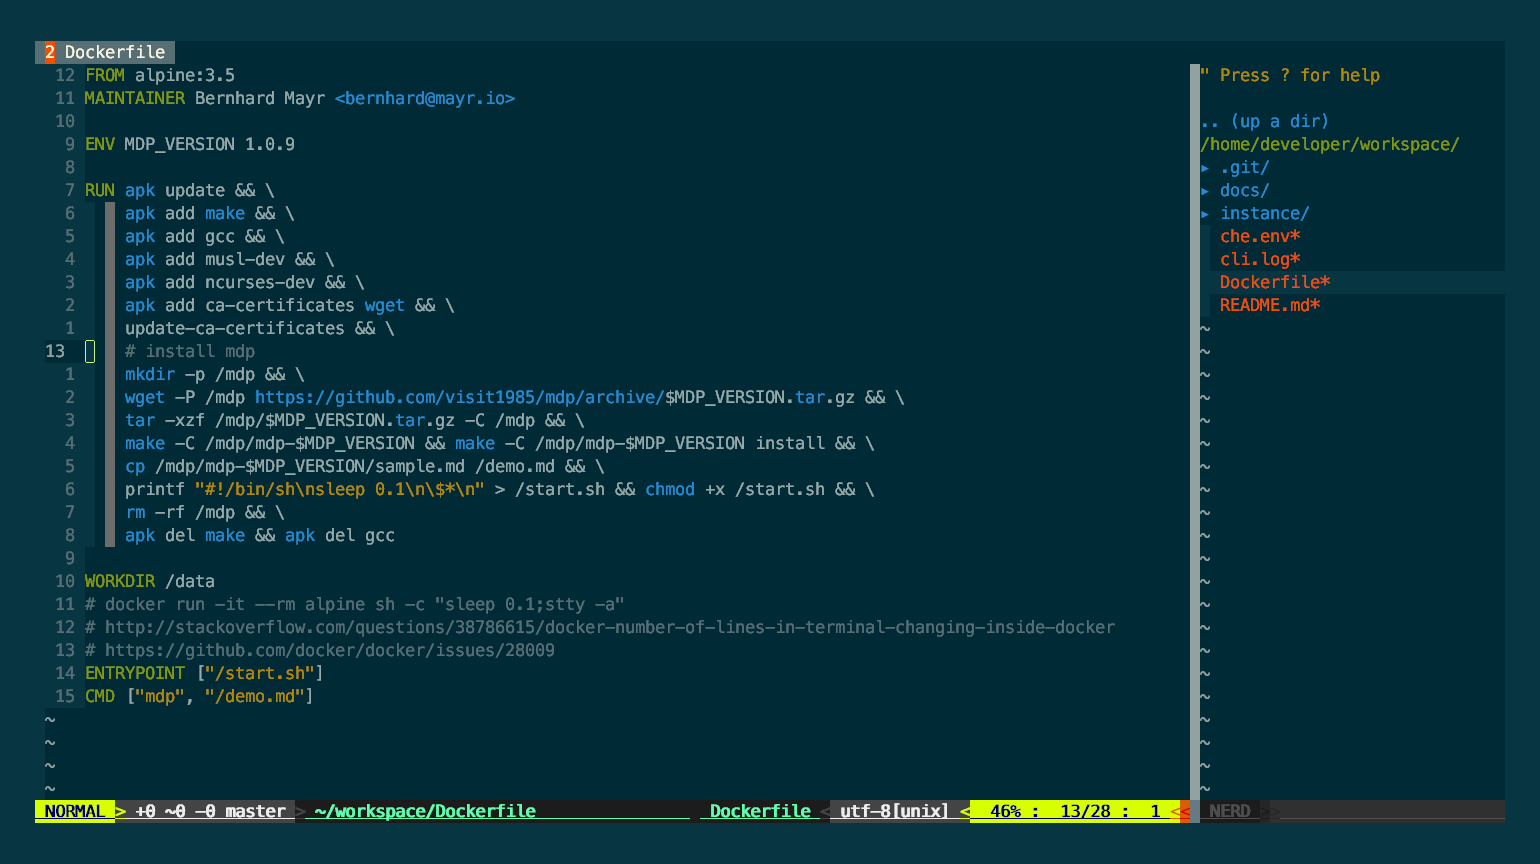
\includegraphics[width=0.8\linewidth,clip]{images/vim-demo}
    \caption{vim als Docker-Container}
\label{fig:vim-demo}
\end{figure}

\subsubsection{Beispiel: Eclipse Che}
\begin{lstlisting}[caption=Docker-Kommando zum Starten von Eclipse Che, language=bash, label=lst:docker-run-eclipse-che]
$ docker run --rm -v /var/run/docker.sock:/var/run/docker.sock -v ${pwd}:/data eclipse/che start
WARN: Bound 'eclipse/che' to 'eclipse/che:5.3.1'
WARN: Did not detect TTY - interactive mode disabled
INFO: (che cli): 5.3.1 - using docker 1.13.1 / docker4windows
INFO: (che start): Booted and reachable
INFO: (che start): Ver: 5.3.1
INFO: (che start): Use: http://10.0.75.2:8080
INFO: (che start): API: http://10.0.75.2:8080/swagger
\end{lstlisting}

\begin{figure}[htbp]
    \centering
    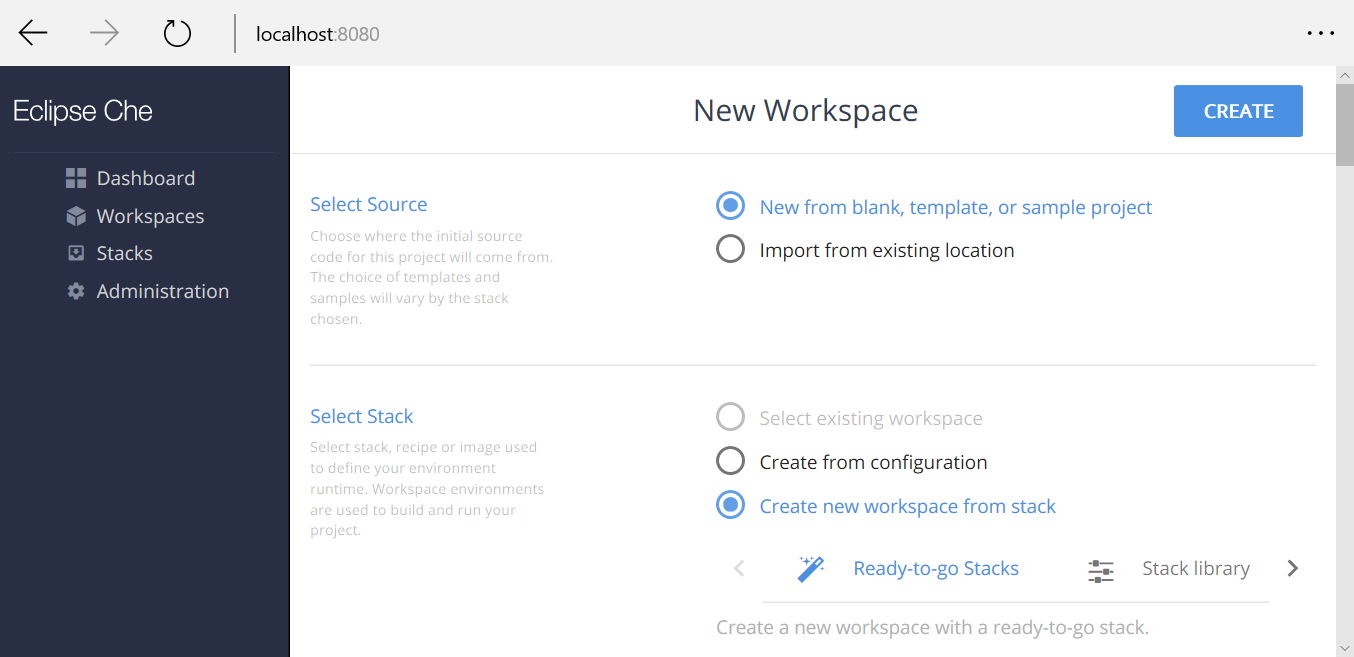
\includegraphics[width=0.8\linewidth,clip]{images/eclipse-che-demo}
    \caption{Eclipse Che als Docker-Container}
\label{fig:eclipse-che-demo}
\end{figure}

% (- https://medium.com/@andyccs/webpack-and-docker-for-development-and-deployment-ae0e73243db4#.dh1mcvvqx)


% ===== EVENTUELL =====
% \section{Docker als Unterstützung zur Entwicklungsumgebung}
% \label{sec:docker-assistance}
%   evtl. SWK6-Umgebung in Docker nachbauen
%   Java, Gradle: http://endoflineblog.com/optimizing-development-with-docker
%   https://blog.nimbleci.com/2016/11/17/whats-coming-in-docker-1-13/
%   http://vuetips.com/use-docker-containers
